\documentclass[11pt]{article}
\usepackage[margin=1in]{geometry}
\usepackage{amsmath,amssymb,amsthm}
\usepackage[hidelinks]{hyperref}
\usepackage{graphicx}

\newtheorem{theorem}{Theorem}
\newtheorem{corollary}{Corollary}
\newtheorem{remark}{Remark}

\newcommand{\eps}{\varepsilon}
\newcommand{\diam}{\operatorname{diam}}
\newcommand{\cnull}{c_0}

\title{A Product Extension of the \(c_0\) Topological CPCP/SR Separation}
\author{Agent lane 17}
\date{2026-06-20}

\begin{document}
\maketitle

\section*{Status}

This is a partial result for the broad question raised by Lopez-Perez and
Medina in \cite{LPM}: starting with a Banach space failing the classical CPCP,
can one build a locally convex topology on its unit ball, containing the weak
topology, such that the unit ball still fails topological CPCP but satisfies
topological strong regularity?

The source paper answers this for \(B_{\cnull}\). The result below extends the
same separation to every \(\ell_\infty\)-sum
\[
   X=\cnull\oplus_\infty Y
\]
with \(Y\) separable.

\section*{Source Question and Input Theorem}

The source paper describes the broad strategy as follows.

\begin{center}
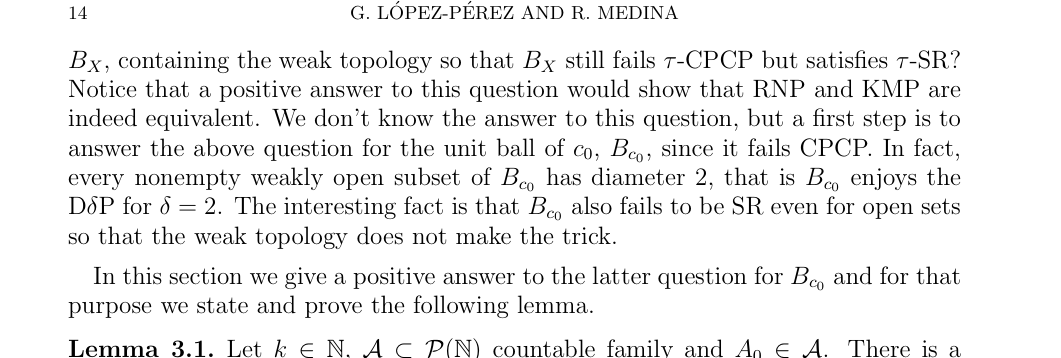
\includegraphics[width=\textwidth]{figures/broad_question_crop.png}
\end{center}

Its key \(c_0\) theorem is \cite[Theorem 3.2]{LPM}.

\begin{center}
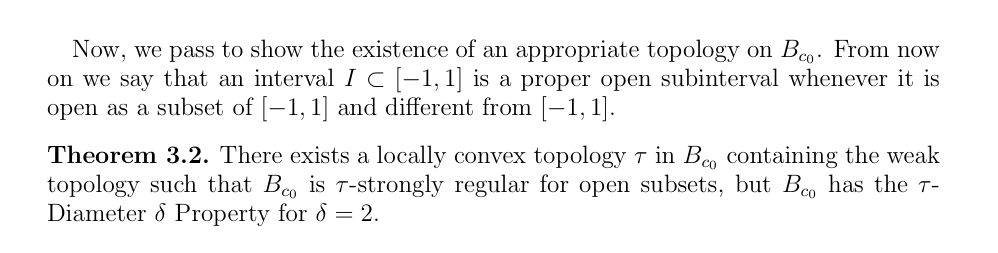
\includegraphics[width=.9\textwidth]{figures/c0_theorem_crop.png}
\end{center}

We use the theorem in the following form. There is a countably based locally
convex topology \(\sigma\) on \(B_{\cnull}\), containing the weak topology, such
that:
\begin{enumerate}
\item every nonempty \(\sigma\)-open subset of \(B_{\cnull}\) has norm diameter
      \(2\);
\item for every nonempty \(\sigma\)-open subset \(U\subset B_{\cnull}\) and
      every \(\eps>0\), \(U\) contains a convex combination of nonempty
      relatively \(\sigma\)-open subsets whose diameter is less than \(\eps\).
\end{enumerate}
The second item is slightly stronger than the formal ``SR for open subsets''
definition, and is exactly what is proved in the last paragraph of
\cite[Theorem 3.2]{LPM}.

\section*{Proof Intuition}

The source construction makes the \(c_0\)-coordinate simultaneously large and
small in two different senses: every open set leaves infinitely many coordinates
free, forcing diameter \(2\), while a later refinement of the subbase supplies
small convex averages inside each open set.

In an \(\ell_\infty\)-sum \(\cnull\oplus_\infty Y\), the \(c_0\)-coordinate
still controls the large-diameter obstruction. To control convex combinations,
put the norm topology on the \(Y\)-coordinate. Then inside any product
neighborhood, choose the source paper's small convex average in \(c_0\) and a
norm-small convex neighborhood in \(Y\). The \(\ell_\infty\)-norm takes the
maximum of the two diameters, so both estimates survive.

\section*{Main Result}

\begin{theorem}
Let \(Y\) be a separable Banach space and let
\[
   X=\cnull\oplus_\infty Y.
\]
Then there is a countably based locally convex topology \(\tau\) on \(B_X\),
containing the weak topology of \(B_X\), such that:
\begin{enumerate}
\item every nonempty \(\tau\)-open subset of \(B_X\) has diameter \(2\);
\item \(B_X\) is \(\tau\)-strongly regular for open subsets.
\end{enumerate}
In particular, \(B_X\) fails \(\tau\)-CPCP while satisfying the topological
strong-regularity conclusion for open subsets.
\end{theorem}

\begin{proof}
Since \(X=\cnull\oplus_\infty Y\), its closed unit ball is the product
\[
   B_X=B_{\cnull}\times B_Y
\]
with norm
\[
   \|(x,y)\|=\max\{\|x\|_{\infty},\|y\|\}.
\]
Let \(\sigma\) be the topology on \(B_{\cnull}\) supplied by
\cite[Theorem 3.2]{LPM}. Define \(\tau\) on \(B_X\) to be the product of
\(\sigma\) on \(B_{\cnull}\) and the norm topology on \(B_Y\). Since \(Y\) is
separable and \(\sigma\) has a countable base, \(\tau\) has a countable base.
It is locally convex. It contains the weak topology on \(B_X\), because
\[
   X^*=(\cnull\oplus_\infty Y)^*=\ell_1\oplus_1 Y^*,
\]
so the weak topology on \(B_X=B_{\cnull}\times B_Y\) is the product of the weak
topologies on the two coordinates; \(\sigma\) contains the weak topology on
\(B_{\cnull}\), and the norm topology on \(B_Y\) contains the weak topology.

Let \(O\) be a nonempty \(\tau\)-open subset of \(B_X\). Choose a nonempty
basic product \(U\times V\subset O\), where \(U\subset B_{\cnull}\) is
\(\sigma\)-open and \(V\subset B_Y\) is norm-open. By the source theorem,
\(\diam(U)=2\). For every \(\eta>0\), choose \(u_1,u_2\in U\) with
\(\|u_1-u_2\|_\infty>2-\eta\), and choose any \(v\in V\). Then
\[
   \|(u_1,v)-(u_2,v)\|=\|u_1-u_2\|_\infty>2-\eta.
\]
Since the diameter of \(B_X\) is \(2\), \(\diam(O)=2\). Thus \(B_X\) fails
\(\tau\)-CPCP already with the convex set \(C=B_X\).

It remains to prove strong regularity for open subsets. Let \(O\) be a nonempty
convex \(\tau\)-open subset of \(B_X\), and let \(\eps>0\). Choose a nonempty
product \(U\times V\subset O\). Shrinking if necessary, assume \(V\) is convex
and has norm diameter less than \(\eps\). By the source theorem, there are
nonempty relatively \(\sigma\)-open subsets \(U_1,\dots,U_m\) of \(U\) and
positive coefficients \(\lambda_1,\dots,\lambda_m\) summing to \(1\) such that
\[
   \diam\left(\sum_{i=1}^m\lambda_i U_i\right)<\eps .
\]
For each \(i\), set \(O_i=U_i\times V\). These are nonempty relatively
\(\tau\)-open subsets of \(O\). Since \(V\) is convex,
\[
   \sum_{i=1}^m\lambda_i O_i
   =
   \left(\sum_{i=1}^m\lambda_i U_i\right)\times V.
\]
Therefore
\[
   \diam\left(\sum_{i=1}^m\lambda_i O_i\right)
   =
   \max\left\{
      \diam\left(\sum_{i=1}^m\lambda_i U_i\right),
      \diam(V)
   \right\}
   <\eps.
\]
This is precisely \(\tau\)-strong regularity for open subsets.
\end{proof}

\begin{corollary}
For every separable Banach space \(Y\), the unit ball of
\(\cnull\oplus_\infty Y\) has a locally convex topology containing the weak
topology for which the topological diameter two property holds while the
corresponding strong diameter two property fails.
\end{corollary}

\begin{proof}
The theorem gives diameter \(2\) for every nonempty \(\tau\)-open subset. It
also gives, inside every nonempty convex \(\tau\)-open subset and for every
\(\eps>0\), a convex combination of relatively \(\tau\)-open subsets with
diameter less than \(\eps\). This is the announced separation.
\end{proof}

\section*{Limitations}

This does not solve the full question from \cite{LPM}: it covers spaces with a
literal \(\ell_\infty\)-summand \(\cnull\), not arbitrary Banach spaces failing
CPCP and not arbitrary spaces merely containing an isomorphic copy of \(c_0\).
The \(\ell_\infty\)-sum norm is used essentially to preserve the diameter
estimate in the \(c_0\)-coordinate and the small-diameter estimate in the
\(Y\)-coordinate by taking a maximum.

\section*{Novelty Check}

Local run indexes were searched for arXiv:2305.18976, CPCP, strong regularity,
Krein--Milman property, and related RNP/KMP terms; no existing packet for this
target was found. Web searches on 2026-06-20 for exact and close phrases
including \texttt{"2305.18976" "c\_0" "locally convex topology"},
\texttt{"CPCP" "strong regularity" "c0" "locally convex topology"}, and
\texttt{"tau-CPCP" "tau-SR" "c\_0"} did not locate a later statement of this
\(\cnull\oplus_\infty Y\) extension. The theorem is best viewed as a short
new product permanence observation built from \cite[Theorem 3.2]{LPM}.

\section*{Human Review Recommendation}

Recommended as a likely valid partial result. The main point to verify is that
the product topology \(\sigma\times\|\cdot\|\) is an admissible locally convex
topology on \(B_{\cnull\oplus_\infty Y}\) containing the weak topology, and
that the product-diameter calculation exactly matches the source definitions
of \(\tau\)-CPCP and \(\tau\)-SR for open subsets.

\begin{thebibliography}{9}

\bibitem{LPM}
G. Lopez-Perez and R. Medina,
\emph{The equivalence between CPCP and strong regularity under Krein-Milman
property},
arXiv:2305.18976, 2023.
\url{https://arxiv.org/abs/2305.18976}

\end{thebibliography}

\end{document}
